% Comments at top of file (fold) 

% This is "sig-alternate.tex" V1.3 OCTOBER 2002
% This file should be compiled with V1.6 of "sig-alternate.cls" OCTOBER 2002
%
% This example file demonstrates the use of the 'sig-alternate.cls'
% V1.6 LaTeX2e document class file. It is for those submitting
% articles to ACM Conference Proceedings WHO DO NOT WISH TO
% STRICTLY ADHERE TO THE SIGS (PUBS-BOARD-ENDORSED) STYLE.
% The 'sig-alternate.cls' file will produce a similar-looking,
% albeit, 'tighter' paper resulting in, invariably, fewer pages.
%
% ----------------------------------------------------------------------------------------------------------------
% This .tex file (and associated .cls V1.6) produces:
%       1) The Permission Statement
%       2) The Conference (location) Info information
%       3) The Copyright Line with ACM data
%       4) NO page numbers
%
% as against the acm_proc_article-sp.cls file which
% DOES NOT produce 1) thru' 3) above.
%
% Using 'sig-alternate.cls' you have control, however, from within
% the source .tex file, over both the CopyrightYear
% (defaulted to 2002) and the ACM Copyright Data
% (defaulted to X-XXXXX-XX-X/XX/XX).
% e.g.
%\CopyrightYear{2005}   %will cause 2002 to appear in the copyright line.
%\crdata{XXX}   %will cause XXX to appear in the copyright line.
%
% ---------------------------------------------------------------------------------------------------------------
% This .tex source is an example which *does* use
% the .bib file (from which the .bbl file % is produced).
% REMEMBER HOWEVER: After having produced the .bbl file,
% and prior to final submission, you *NEED* to 'insert'
% your .bbl file into your source .tex file so as to provide
% ONE 'self-contained' source file.
%
% ================= IF YOU HAVE QUESTIONS =======================
% Questions regarding the SIGS styles, SIGS policies and
% procedures, Conferences etc. should be sent to
% Adrienne Griscti (griscti@acm.org)
%
% Technical questions _only_ to
% Gerald Murray (murray@acm.org)
% ===============================================================
%
% For tracking purposes - this is V1.3 - OCTOBER 2002

% Comments at top of file (end) 

\documentclass{NIME-alternate}
\usepackage{hyperref}
\usepackage{url}
\usepackage{color}
\definecolor{black}{rgb}{0,0,0}
\hypersetup{colorlinks
,linkcolor=black
,filecolor=black
,urlcolor=black
,citecolor=black}
%reduces the space between the items in the itemize-environment 
\newenvironment{packed_item}{
\begin{itemize}
  \setlength{\itemsep}{1pt}
  \setlength{\parskip}{0pt}
  \setlength{\parsep}{0pt}
}{\end{itemize}}


\begin{document}

% Title part (fold) 
%
% --- Author Metadata here ---
\CopyrightYear{2008}   %will cause 2008 to appear in the copyright line.
\crdata{Copyright remains with the author(s).}
\conferenceinfo{NIME08,}{ Genova, Italy}
%\CopyrightYear{2001} % Allows default copyright year (2000) to be over-ridden - IF NEED BE.
%\crdata{0-12345-67-8/90/01}  % Allows default copyright data (0-89791-88-6/97/05) to be over-ridden - IF NEED BE.
% --- End of Author Metadata ---

\title{Differentiating Values and Properties in OSC}
% CHANGED: Added subTitle [TAP]
\subtitle{Addressing Classes with Open Sound Control}

%
% You need the command \numberofauthors to handle the "boxing"
% and alignment of the authors under the title, and to add
% a section for authors number 4 through n.
%
% Up to the first three authors are aligned under the title;
% use the \alignauthor commands below to handle those names
% and affiliations. Add names, affiliations, addresses for
% additional authors as the argument to \additionalauthors;
% these will be set for you without further effort on your
% part as the last section in the body of your article BEFORE
% References or any Appendices.

\numberofauthors{5}
%
% You can go ahead and credit authors number 4+ here;
% their names will appear in a section called
% "Additional Authors" just before the Appendices
% (if there are any) or Bibliography (if there
% aren't)

% Put no more than the first THREE authors in the \author command
\author{
% The command \alignauthor (no curly braces needed) should
% precede each author name, affiliation/snail-mail address and
% e-mail address. Additionally, tag each line of
% affiliation/address with \affaddr, and tag the
%% e-mail address with \email.
\alignauthor Timothy Place \\
	\affaddr{Electrotap}\\
	\affaddr{6920 N. Mercier Street}\\
	\affaddr{Kansas City, Missouri 64118}\\
	\affaddr{USA}\\
	\email{tim@electrotap.com}
\alignauthor Trond Lossius \\
	\affaddr{BEK - Bergen Center for Electronic Arts}\\
	\affaddr{C. Sundtsgt. 55}\\
	\affaddr{N-5004 Bergen, Norway}\\
	\email{lossius@bek.no}
\alignauthor Alexander Refsum Jensenius \\
	\affaddr{University of Oslo}\\
	\affaddr{PB 1017 Blindern}\\
	\affaddr{N-0315 Oslo, Norway}\\
	\email{a.r.jensenius@imv.uio.no}
}
% FIXME: the additional authors are not showing up in the paper -- why?
\additionalauthors{
	Additional authors: Nils Peters (McGill University, email: {\texttt{nils.peters@mcgill.ca}}) 
   and Pascal Baltazar (GMEA, email: {\texttt{pb@gmea.net}}).
}


%%%%%%%%%%%%%%%%
\maketitle

% Title part (end) 

% Hyphenations (fold)
\hyphenation{ja-mo-ma}
% Hyphenations (end)

\begin{abstract}

An approach for creating structured Open Sound Control (OSC) messages by separating the addressing of node \emph{values} and node \emph{properties} is suggested. This includes a method for querying values and properties. As a result, it is possible to address complex nodes inside of more complex tree structures using an OSC namespace. This is particularly useful for creating flexible communication in modular systems.  A prototype implementation is presented and discussed.

\end{abstract}

\keywords{OSC, namespace, Jamoma, standardization}


%%%%%%%%%%%%%%%%%%%%%%
%%%%%%%%%%%%%%%%%%%%%%
%%%%%%%%%%%%%%%%%%%%%%

\section{Introduction} % (fold)
\label{sec:introduction}

Open Sound Control (OSC)\footnote{\url{http://www.opensoundcontrol.org}} has evolved into the de facto standard in the computer music community for communication in and between controllers and sound engines \cite{Wright:2003}. OSC is a protocol for transmitting messages where the addressing of nodes is based on a ``slash'' notation similar to URLs. As such, OSC is focused on standardizing the communication of messages, but there is no prescribed standardization of the namespaces or the structure of these namespaces. 

The authors are involved in developing OSC namespaces for the Jamoma\footnote{\url{http://www.jamoma.org}} project. Jamoma is a modular system for developing high-level modules in the Max/MSP/Jitter environment. It uses OSC for internal and external communication \cite{Place:2006}.  As Jamoma's modular structures grow more complex, we find the bi-dimensional namespace conventions of OSC to be inadequate for addressing our constructs.  OSC standardizes the addressing of a node, but it becomes increasingly unclear what to do once we reach the node.  The problem is exacerbated when the node itself implements its own OSC namespace, as is the case with Jamoma.

% CHANGED: Added Bibdesk reference to the spec itself, and cite it. [TL]

The OSC 1.0 specification \cite{Wright:2002} consider nodes only in terms of their methods: ``OSC Methods are the potential destinations of OSC messages received by the OSC server and correspond to each of the points of control that the application makes available. `Invoking' an OSC method is analogous to a procedure call; it means supplying the method with arguments and causing the method's effect to take place.'' 

This paper extends current OSC concepts by considering nodes to represent classes in an object-oriented sense, rather than simple methods.  For the purposes of this discussion, we will be considering only nodes that contain one or more methods and/or properties.   Properties provide additional information concerning how the node behaves and responds to methods, e.g. by specifying \emph{how} a parameter interpolates to a new value. A node might or might not have a value. If it does possess a value property, that value may be set directly, as it is considered an implicit property of the node. A node may branch out to additional nodes, as in existing OSC practice.

The paper starts by reviewing various approaches to creating more complex communication using OSC. This is followed by a presentation and discussion of our suggested approach, introducing the use of a colon for separating between values and properties. Finally, a prototype implementation built in Jamoma is presented and discussed. 

% section introduction (end)



%%%%%%%%%%%%%%%%%%%%%%
%%%%%%%%%%%%%%%%%%%%%%
%%%%%%%%%%%%%%%%%%%%%%

\section{Complex Structures in OSC} % (fold)
\label{sec:complex_structures_in_OSC}


The original idea of OSC is that it is tree-structured into a hierarchy called the \emph{address space} where each of the nodes has a symbolic name and is a potential destination of OSC messages \cite{Wright:1997}. In contrast to the static schema of MIDI, the \emph{open} nature of OSC means that the address space is defined and created by the ``implementor’s idea of how these features should be organized'' \cite[p153]{Wright:2003}.

%CHANGED: Don't really see what the example adds to the discussion, so it's commented out. [TL]

%For example: 
%
%\noindent
%\texttt{/voices/3/freq 440.0}

This open approach has made OSC useful in a broad range of applications, and adaptable to situations not foreseen by its developers \cite{Wright:2005}.  However, this lack of standardization in namespace schemas is also likely a major reason that OSC has not gained more widespread use in commercial software applications.


%%%%%%%%%%%%%%%%%%%%%%

\subsection{OSC Namespace Standardization} % (fold)
\label{sub:namespace_standardization}

A growing expanse of projects, including the research on mapping between controllers and sound engines, require the ability to discover and query namespaces using a known and common syntax \cite{Malloch:2007}. Other projects, such as LIBOSCQS\footnote{\url{http://liboscqs.sourceforge.net}} attempt to solve the problem of disparate namespaces by providing a query system and service discovery for applications using the OSC protocol \cite{Habets:2005, Schmeder:2004oscqs}.

%\noindent \textbf{Occam} takes OSC messages and converts them to MIDI. It exports a MIDI source to CoreMIDI which can be used in any Mac OS X application that accepts MIDI. It broadcasts the existence of this OSC-to-MIDI service using Rendezvous (Zero-Conf).\\    

%\textbf{Iannix} \footnote{\url{http://sourceforge.net/projects/iannix}} is a graphical editor of multidimensional and multi-formal scores, a kind of poly-temporal meta-sequencer, based on the former UPIC created by Iannis Xenakis." The current implementation is built around a client/server model where all communication is handled using OSC. \cite{Coduys:2004}\\

Several projects have undertaken a standardization of OSC messages, and OSC syntax, for different purposes. In actual practice, these various independent efforts at standardizing namespaces incorporate syntactic elements with conflicting meanings as compared to each other. However, there are some commonalities to these efforts and the problems that they try to address.

\subsubsection{Querying Nodes}
A primary concern in many of these efforts is the ability to query a node for it's value. The Integra project\footnote{\url{http://www.integralive.org}} uses a \texttt{.get} appended to the node's address
% CHANGED: This does not build our argument, so I cut it as previously discussed [TAP]
%\footnote{Integra also suggests using the : (colon) to set messages without outputting, to avoid feedback.}. 
Meanwhile JazzMutant's OSC 2.0 Draft Proposal suggests repurposing the reserved \texttt{?} to query for the value of a node %\cite{Jazzmutant:2006} 
%CHANGED: I took the first jazzmutant cite out, because it is not very neccesary and just needs spacce at the end. [NP]
\cite{Jazzmutant:2007}. We agree that this functionality is needed, and that a standardized way of doing it is essential.  However, we propose that users are interested not only in querying the value of the node, but other properties of that node as well.

\subsubsection{Specifying Additional Information}
The standardization of OSC namespaces for interfacing with VST Plug-ins was suggested in \cite{Zbyszynski:2005}, where units may be specified for the value that is being sent to or from a node.  In this proposal the units are specified within the namespace.  For example, \texttt{/low/output} and \texttt{/low/dBoutput} are two ways of controlling the same thing (gain) but specified using different units. This is a similar approach as to how we have previously addressed different types of units in Jamoma, e.g. for specifying gain in either MIDI (\texttt{/audio/gain/midi}) or dB (\texttt{/audio/gain}).\\ 
While such an approach may be beneficial in some contexts, we find that a more structured approach could be beneficial in more complex setups. We therefore propose that the units should be specified as a property of that node rather than contaminating the namespace itself.

\subsubsection{Augmented Syntax}

A review of the myriad of attempts at creating standardized OSC schemas, and standardized means of discovering and querying namespaces, indicates that additional syntax is needed for clarifying function, address, or both when working with a complex OSC system.  Integra, JazzMutant, and Jamoma are all examples where additional symbols, such as the colon, have reserved (if different) meanings.

To investigate possible alternatives for sending this structured information, it is useful to observe the fundamentals of other existing methodologies for representing and sending data over a network.

% TODO: The following seems obsolete now because of the mzed citation.  Figure out if we need this somewhere.  If not, delete. Alexander: Since we include the temperature example in the XML section, it could be good to keep it here?
%In Jamoma, a wide variety of cases exist where a value may be set for a given node in the OSC namespace. However, the node also has additional properties which define the behavior of that node.  For example, a node may represent the temperature such as:
%
%\texttt{/path/to/the/temperature 32}
%
%However, we may wish to set a property of the node so that it knows how to interpret the temperature.  Is it specified in Celsius or Fahrenheit?  Is this a shift from an existing value, or is setting the value directly?  Before we send the value, perhaps we should query the node to find out what an acceptable range is for this node.
%
%This problem of accessing properties of a node, as opposed to the value of a node, is particularly troublesome using the standard OSC addressing conventions (using only slashes to navigate the tree).  One example of a system parallel to OSC for representing and sending data over a network is XML.

% subsection namespace_standardization (end)

%%%%%%%%%%%%%%%%%%%%%%

\subsection{XML} % (fold)
\label{sub:xml}

Extensible Markup Language (XML)\footnote{\url{http://www.w3.org/XML/}} is a particularly relevant analogue to OSC.  XML defines a means for formatting data, but not the data or anything specific to the dataspace itself \cite{xml:2006}. 

A number of standardized namespaces using XML have gained wide adoption, including Scalable Vector Graphics (SVG)\footnote{\url{http://www.w3.org/Graphics/SVG/}}, XHTML\footnote{\url{http://www.w3.org/TR/xhtml1/}} and SOAP\footnote{\url{http://www.w3.org/TR/soap/}}.  SOAP is of particular interest because it is designed as a protocol for exchanging structured information.

Using XML, information is encapsulated into elements.  These elements form a tree structure analogous to an OSC message, and for the purpose of this discussion we will treat them as such.  Using XML elements, one way to represent the preceding audio gain example is thus:
%\begin{small}
%\begin{verbatim}
%<path><to><gain> 0 </gain></to></path>
%\end{verbatim}
%\end{small}

\texttt{<audio><gain> 0 </gain></audio>}

This is clearly more cumbersome to manually type this XML than the equivalent OSC message:

\texttt{/audio/gain 0}

It is also more work for the receiving processor to parse, and it uses more bandwidth as well.\footnote{The Efficient XML Interchange (EXI) Format solves many of these concerns with XML, but at the expense of human readability because it is a binary format.  \url{http://www.w3.org/TR/2007/WD-exi-20071219/}} However, XML elements are able not only to express a value (\emph{content} in xml parlance) between the tags, but also they can provide properties (\emph{attributes}) to the node. For example, we may provide the unit for specifying the gain:
%\begin{small}
%\begin{verbatim}
%<path><to><gain unit=`dB'> 0 </gain></to></path>
%\end{verbatim}
%\end{small}

\texttt{<audio><gain unit=`dB'> 0 </gain></audio>}

We suggest a model where it is possible to fork an OSC address to access not only the value of the node, but also the properties of that node, much like what is possible in other existing models such as XML\footnote{A more concise option than XML, albeit with less clarity and interoperability than OSC, is JSON (\url{http://www.json.org})}.  

% CHANGED: I'm not sure if we really need this, so I'm commenting out for now [TAP]
%Different than XML, we will propose that they can be addressed independently rather than simultaneously in.

% subsection xml (end)

\subsection{OSC Nodes as Classes} % (fold)
\label{sub:osc_nodes_as_classes}

In the introduction we made reference to the OSC 1.0 Specification, which states an OSC node represents a function call on a server. We propose that OSC nodes may represent more complex classes, and thus require a mechanism to address the members of these classes. A class \emph{member} may be a \emph{property} or a \emph{method}.

In the Figure~\ref{fig:paths}, the OSC namespace from the previous examples is shown across the x-axis. Traversing the OSC namespace is an action making a horizontal traversal across the figure.  In the next section, we will suggest a new syntax for traversing this diagram on the y-axis to address the members inside of these nodes.

\begin{figure}
\centerline{\framebox{
	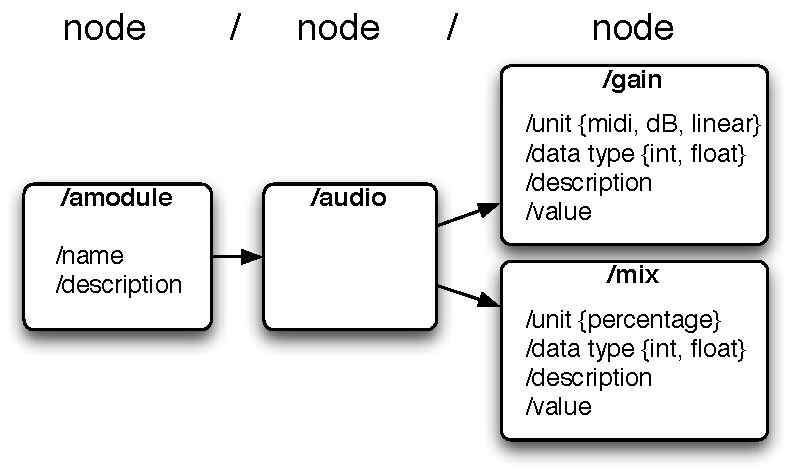
\includegraphics[width=\columnwidth]{figure-paths}}}
\caption{An OSC address tree, with some nodes as classes}
\label{fig:paths}
\end{figure}

% subsection osc_nodes_as_classes (end)


\subsection{Introducing the Colon Separator} % (fold)
\label{sub:the_colon_separator}

In addition to the ASCII symbols already reserved for specific purposes within the OSC protocol \cite{Wright:1997}, we introduce the colon ``\texttt{:}'' as a separator between the OSC address of a node and the namespace for accessing the members of the node:

\texttt{<node address> <value>}

\texttt{<node address>:<member address> <value>}

The former message sets the value of the node just as it would using the existing OSC conventions. This is because a property named \emph{value} is considered to be implicitly addressed if there is no specific member address given. The latter form calls or sets a member of the node.  The member itself is addressed using a fully-qualified OSC namespace. Again using gain as an example, we can send two messages: one for setting the unit property and one for setting the value.

\texttt{/module/audio/gain:/unit midi}

\texttt{/module/audio/gain 120}

%This usage of the colon has precedent in POSIX paths when addressing remote filesystems.  For example, scp uses the following format to locate a file on a remote server:

% TODO: This is actually weakening our argument, we aren't using the colon like this at all.  It's better to use the diagram with / traversing horizontally and the colon to traverse vertically. [TAP]
% CHANGED: Agrees with Tim, commenting it out. [TL]
%\texttt{user@host.com:/path/to/file}

%In our case, we are indeed using the colon to separate OSC namespaces, one of which is the address to a node and one of which is the address within that remote node.  By reserving the colon for this usage, we also make the strings both fast and easy to parse.

Section~\ref{sec:prototype_implementation} provides an illustration of the ideas suggested here. In the remainder of the discussion, the address of the node will be omitted for the sake of brevity; e.g.\\ 
\texttt{/computer/module/parameter:/member}  
will be abbreviated as \texttt{:/member}.

% subsection the_colon_separator (end)


\subsection{Standardizing Members} % (fold)
\label{sub:standardizing_members}

To make working with classes in OSC practical, it is important to have some standard members in place. At present we recommend standardizing the following member methods, and reserving their syntax:
\begin{packed_item}%\begin{itemize}
	\item \texttt{:/get} returns the value of the node.
	\item \texttt{:/dump} returns the state of the node, which is to say the values of all of the properties including the value itself.
	\item \texttt{:/namespace} returns the namespace implemented at this node.
	\item \texttt{:/catalog} returns an enumeration of available options for a node, if relevant.
\end{packed_item}%\end{itemize}

% subsection standardizing_members (end)

% section complex_structures_in_OSC (end)


%%%%%%%%%%%%%%%%%%%%%%
%%%%%%%%%%%%%%%%%%%%%%
%%%%%%%%%%%%%%%%%%%%%%

\section{A Prototype Implementation} % (fold)
\label{sec:prototype_implementation}

The general concepts introduced in this paper form the basis of the standardized namespace for node members used in Jamoma. The following uses select aspects of the Jamoma node namespace to illustrate how class-oriented addressing in OSC can provide users with extended and structured control of available nodes.

Jamoma distinguishes between the \emph{parameters} and \emph{messages} of a module.  Both parameters and messages are addressed as OSC \emph{nodes}. The primary difference is that parameter nodes implement a value property.  The remaining properties of these nodes are shared.


%%%%%%%%%%%%%%%%%%%%%%

\subsection{Node Type} % (fold)
\label{sub:type}

The type of the node can be specified. Possible types are \emph{none}, \emph{boolean}, \emph{integer}, \emph{float32}, \emph{symbol} and \emph{list}. If one do not want to restrict the type of the node, it can be set to \emph{generic}. The \emph{none} type is only valid for messages. Some of the properties below will only be valid for certain types of nodes. The type property is accessed thus:

\begin{tabular}{ll}
	\texttt{:/type} & \texttt{:/type:/get} \\
\end{tabular}

% subsection type (end)


%%%%%%%%%%%%%%%%%%%%%%

\subsection{Controlling the Node Itself} % (fold)
\label{sub:controlling_the_node_itself}

As the node value is concidered an implicit property, it can be set and retrieved as such. If the node is an integer, float or list type it can also be stepwise increased or decreased. If so the size of the steps is itself a property:

\begin{tabular}{ll}
	\texttt{:/value} & \texttt{:/value:/get} \\
	\texttt{:/value/stepsize}  & \texttt{:/value/stepsize:/get} \\
	\texttt{:/value/inc} \\
	\texttt{:/value/dec} \\
\end{tabular}

% subsection controlling_the_node_itself (end)



%%%%%%%%%%%%%%%%%%%%%%

\subsection{Controlling the Range} % (fold)
\label{sub:range}

For integer, float and list nodes a range can be specified. This can be useful for setting up autoscaling mappings from one value to another, or for clipping the output range. The clipping property can be \emph{none}, \emph{low}, \emph{high} or \emph{both}. The range properties are accessed thus:

\begin{tabular}{ll}
	\texttt{:/range/bound} & \texttt{:/range/bound:/get} \\
	\texttt{:/range/clipmode}  & \texttt{:/range/clipmode:/get} \\
\end{tabular}

% subsection range (end)



%%%%%%%%%%%%%%%%%%%%%%

% CHANGED: Left out to save space.

%\subsection{Filtering of Repetitions} % (fold)
%\label{sub:filtering_of_repetitions}
%
%It is sometimes useful to filter repetitions to avoid redundant processing. The \emph{boolean} repetitions property is accessed thus:
%
%\begin{tabular}{ll}
%	\texttt{:/repetitions} & \texttt{:/repetitions:/get} \\
%\end{tabular}
%
% subsection filtering_of_repetitions (end)



%%%%%%%%%%%%%%%%%%%%%%

\subsection{Ramping to New Values} % (fold)
\label{sub:ramping_to_new_values}

The ability to smoothly move from one value to another is fundamental to any kind of transition and transformation of musical or artistic material. Jamoma offers the possibility of interpolating from the current to a new value in a set amount of time. While the OSC message

\texttt{/myComputer/myModule/myParameter 1.0}

\noindent
will set the parameter value to $1.0$ immediately, the message

\texttt{/myComputer/myModule/myParameter 1.0 ramp 2000}

\noindent
will cause the value to interpolate, or ramp, to $1.0$ over 2000 milliseconds. Ramping in Jamoma works with messages and parameters of type integer, float and list.

Jamoma offers vastly extended possibilities in how ramping can be done as compared to Max. In Jamoma the process of ramping is made up from the combination of two components: A \emph{drive} mechanism triggers calculations of new values at desired intervals during the ramp, while a set of \emph{functions} offers a set of curves for the ramping. Libraries for both components are implemented as C++ APIs, and can easily be extended.


\subsubsection{Ramp Drive} % (fold)
\label{ssub:the_ramp_lib}

The ramp drive in Jamoma is implemented as a library of self-contained classes, coined \emph{RampUnits}.  The existing classes include a \emph{scheduler} drive using the Max scheduler, a \emph{queue} drive running in the Max queue, and an \emph{async} drive which calculates output only when an update is requested.

% CHANGED: Abbreviated to save space, the details are left for the ICMC paper.

% When a new ramp is started, the \emph{RampUnit} internally uses a normalized ramping value, increasing linearly from $0.0$ to $1.0$ over the duration of the ramp. When the RampUnit is to provide a new value, it updates the normalized ramping value, and passes it to a FunctionUnit as described in Section~\ref{ssub:the_function_lib}. The normalized value returned is then scaled to the range defined by the start and end values for the ramp, and the node's value is updated.

The ramp units internally perform normalized linear ramps. The values are then mapped and scaled using the appropriate FunctionUnit as discussed in Section~\ref{ssub:the_function_lib}. 

% subsubsection the_ramp_lib (end)


\subsubsection{Ramp Function} % (fold)
\label{ssub:the_function_lib}

The ramp function in Jamoma is handled by the Jamoma \emph{FunctionLib}.  The FunctionLib provides normalized mappings of values $x \in [0,1]$ to $y \in [0,1]$ according to functions $y = f(x)$. Currently five \emph{FunctionUnits} are implemented: Linear, cosine, lowpass series, power function and hyperbolic tangent. There are plans to expand this additional functions.

% subsubsection the_function_lib (end)


\subsubsection{OSC Namespace for Ramping Properties} % (fold)
\label{ssub:osc_namespace_for_ramping_properties}
Ramping properties are addressed using \texttt{:/ramp/drive} and \texttt{:/ramp/function} OSC name classes. The ramping case provides an example of a node class which contains other node classes, as illustrated in Figure~\ref{fig:embedded}. In to setting or getting the current ramp drive mechanism, the ramp drive mechanism may itself have parameters. It is also possible to have the module return a list of all available ramp units, implemented with the standardized \texttt{:/catalog} message.

\begin{figure}
\centerline{\framebox{
	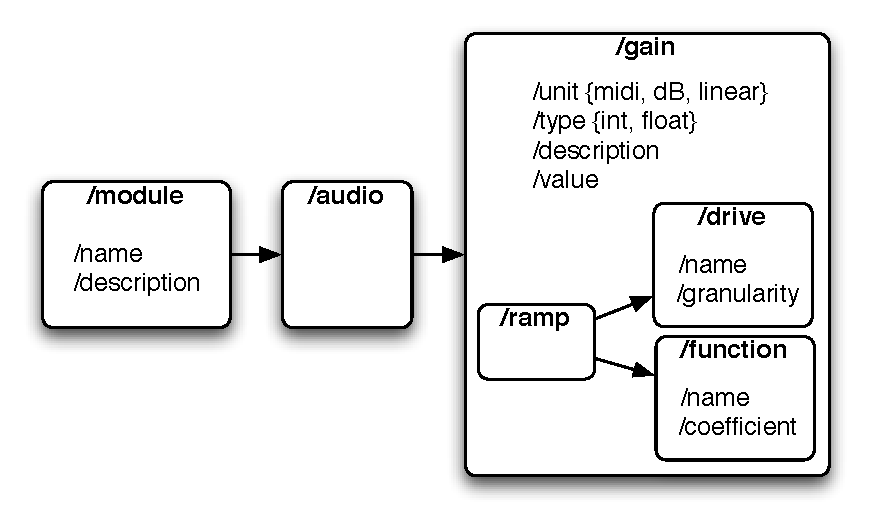
\includegraphics[width=\columnwidth]{figure-embedded}}}
\caption{An example OSC address tree to nodes within another node}
\label{fig:embedded}
\end{figure}


\begin{tabular}{ll}
	\texttt{:/ramp/drive} & \texttt{:/ramp/drive:/get} \\
	\texttt{:/ramp/drive:/catalog} \\
	\texttt{:/ramp/drive:/dump} \\
	\texttt{:/ramp/drive:/namespace} \\
	\texttt{:/ramp/drive:/catalog} \\
	\texttt{:/ramp/function}  & \texttt{:/ramp/function:/get} \\
	\texttt{:/ramp/function:/catalog} \\
	\texttt{:/ramp/function:/dump} \\
	\texttt{:/ramp/function:/namespace} \\
\end{tabular}

RampUnits that have additional parameters can be investigated with the \texttt{:/namespace} method. Those parameters are then addressed as properties of the ramp/drive or ramp/function nodes.  For instance the user can control how often the \emph{scheduler} RampUnit is to update by setting the \texttt{:/granularity} property of the ramp:

\texttt{:/ramp/drive:/granularity}

\texttt{:/ramp/drive:/granularity:/get}

The same principles apply to the function used for ramping. 

% subsubsection osc_namespace_for_ramping_properties (end)



% subsection ramping_to_new_values (end)



%%%%%%%%%%%%%%%%%%%%%%

\subsection{Description} % (fold)
\label{sub:description}

The description property is a string providing a text description of the parameter. In Jamoma this is used for auto-generating online documentation of the modules. It can also be used for building modules that retrieve the total namespace of all Jamoma modules used, and provide interactive documentation of available parameters. The descriptions property is accessed as:

\begin{tabular}{ll}
	\texttt{:/description} & \texttt{:/description:/get} \\
\end{tabular}

% subsection description (end)


% section prototype_implementation (end)



%%%%%%%%%%%%%%%%%%%%%%
%%%%%%%%%%%%%%%%%%%%%%
%%%%%%%%%%%%%%%%%%%%%%

\section{Discussion and Further Work} % (fold)
\label{sec:discussion_and_further_work}   


\subsection{DataspaceLib} % (fold)
\label{sub:dataspacelib}

In addition to the current RampLib and FunctionLib, work has started on the implementation of a DataspaceLib.  The DataspaceLib enables nodes to be addressed using one of several interchangeable measuring units. For example a gain parameter can be set using MIDI, dB or linear amplitude depending on the context and preferences of the user. The OSC representation of this is implemented as a set of properties to the node. The DataspaceLib is also meant to offer mapping between more complex interrelated coordinate systems, so that e.g. cartesian and spherical coordinates can be used interchangeably for description of points in space.

%TODO: Insert bib ref to the SpatDIF paper by Nils Peters

% subsection dataspacelib (end)


Querying - we propose a different system to the JazzMutant OSC2 draft

Expanding :/dump for namespace discovery

In the figure the slash equals stepping in the right direction, to the next branch of the OSC namespace, while the colon indicates stepping downwards in order to access the inner properties of the current node.

Use analogy: what we are doing is really similar to C++ classes.

The proposal set forward in this paper could be cosidered one step in the direction of a more object oriented approach to Open Sound Control

% section discussion_and_further_work (end)




%\end{document}  % This is where a 'short' article might terminate



%%%%%%%%%%%%%%%%%%%%%%
%%%%%%%%%%%%%%%%%%%%%%
%%%%%%%%%%%%%%%%%%%%%%

%ACKNOWLEDGMENTS are optional
\section{Acknowledgments} % (fold)
\label{sec:acknowledgments}

The authors would like to thank all Jamoma developers and users for valuable contributions, and iMAL Center for Digital Cultures and Technology for organizing a workshop where the issues presented in this paper were discussed.

% section acknowledgments (end)



%%%%%%%%%%%%%%%%%%%%%%
%%%%%%%%%%%%%%%%%%%%%%
%%%%%%%%%%%%%%%%%%%%%%

% Bibliography (fold)
%
% The following two commands are all you need in the initial runs of your .tex file to
% produce the bibliography for the citations in your paper.
\begin{small}
\bibliographystyle{abbrv}
\bibliography{jamoma-nime2008}  % the name of the Bibliography in this case
\end{small}
% You must have a proper ".bib" file
%  and remember to run:
% latex bibtex latex latex
% to resolve all references
%
% Bibliography (end)


\balancecolumns % GM July 2000
% That's all folks!
\end{document}
